\documentclass[onecolumn]{article}
%\usepackage{url}
%\usepackage{algorithmic}
\usepackage[a4paper]{geometry}
\usepackage{datetime}
\usepackage[margin=2em, font=small,labelfont=it]{caption}
\usepackage{graphicx}
\usepackage{mathpazo} % use palatino
\usepackage[scaled]{helvet} % helvetica
\usepackage{microtype}
\usepackage{amsmath}
\usepackage{subfigure}
% Letterspacing macros
\newcommand{\spacecaps}[1]{\textls[200]{\MakeUppercase{#1}}}
\newcommand{\spacesc}[1]{\textls[50]{\textsc{\MakeLowercase{#1}}}}

\title{\spacecaps{ Using Multilayer Perceptron and Levenberg-Marquardt Algorithm to Predict Forest Fires}\\ \normalsize \spacesc{CENG3521, Data Mining} }

\author{Ali Akgöl\\aliakgol@posta.mu.edu.tr \\\\ Sultan Güvenbaş\\ sultanguvenbas@posta.mu.edu.tr}
\date{}


\begin{document}
\maketitle

\section{Abstract}
Forest fires are crucial events that affect both human lives and environment and create many damages especially in recent decades. There are many reasons to break out forest fires. Some of them are on purpose and some of them are happened by carelessness. To decrease the damage of forest fires and if possible, prevent from forest fires, many studies have been done to detect forest fires by using machine learning methods. The aim of this study is to predict the forest fires to decrease the harm that would occur by these fires. In [1], different machine learning methods including Multilayer Perceptron (MLP) have been used to detect the forest fires; however, in this study We are planning to apply MLP with more than one hidden layer and different activation function and also apply to Levenberg-Marquardt (LM) algorithm to predict forest fires and compare the result with the study of [1]. The RMSE (Root mean square error) values of the models have been computed to determine the performance of the forest fires prediction models.
\\
\\
\textbf{Keywords-} Forest Fires, Multi Layer Perceptron, Portugal,Levenberg-Marquardt Algorithm

\section{Introduction}
One of the important environmental disasters is forest fire. Forest fires create damages in ecological system, in addition to threaten people’s lives. The reasons of the forest fires are whether human activity or environmental disasters. The forest fires occurred by human can be separated into two groups such as on purpose or accidentally. The fires, that happened accidentally, occurred inattention behaviors of humans that have a picnic or hunters. The fires, that happened on purpose, occur by destruction of forest or shrubs to use destructed land for agricultural activities etc. [2]. Another factor for the forest fires happened on fires is alteration on climates; that is, higher temperature or less rain which can be explain with global warming [3]. 
Forest fires harm human’s life as well as land; that is why, they cost so much and are very hazardous. Thus, predicting forest fire earlier is very important to save many human’s life and also lots of resource of the land. In other words, if the forest fire is realized at the start, then it can be prevented growth of the fire.
The aim of this project is to extend the work to predict the forest fires to decrease the harm that would occur by these fires. 

In literature, it has been done many re-searches upon forest fires all around the world. Many of these re-searches has been done by using Artificial Neural Network (ANN) in Wireless Sensor Network (WSN). However, lately, Convolutional Neural Network (CNN) has been applied as well as ANN.
In [4], WSN has been combined with ANN to find a smart system to detect forest fires. By this system, authors aimed to decrease the cost that resulted from forest fires. While data has been collected, there main points have been considered which are smoke, temperature, and light in [4].
In [5], authors have been applied ANN to indicate which areas are risky according to the forest fires at most. They have been used data set which had been collected from different locations of Brazilian in 2005 in [5]. These locations are generally agricultural areas. 


\section{Dataset Attribute Information}
The dataset has been used in this study has been collected from a natural park which name is Montesinho from the northeast area of Portugal. The map of the park is given by Fig.1. Many species of plants and animals are existed in this park. The temperature has been changed on average between 8 and 12 ◦C annually in this park. The data had been started to collect from January 2000, until the end of December 2013[1].
The inputs used in the data set is described in Table 1. Four FWI(FFMC,DMC,DC,ISI) gives the weather conditions. However, since FWI is dependent to the former values, it has discarded[1]. We also did not use day attribute as well.
\begin{figure}[htb!]
\centerline
{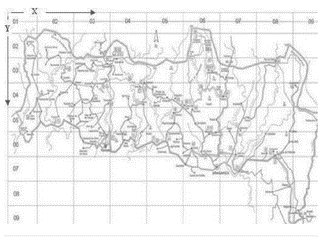
\includegraphics[width=105mm,scale=1.0]{fig1.png}}
\caption{The map of Montesinho natural park}
\end{figure}

\begin{figure}[htb!]
\centerline
{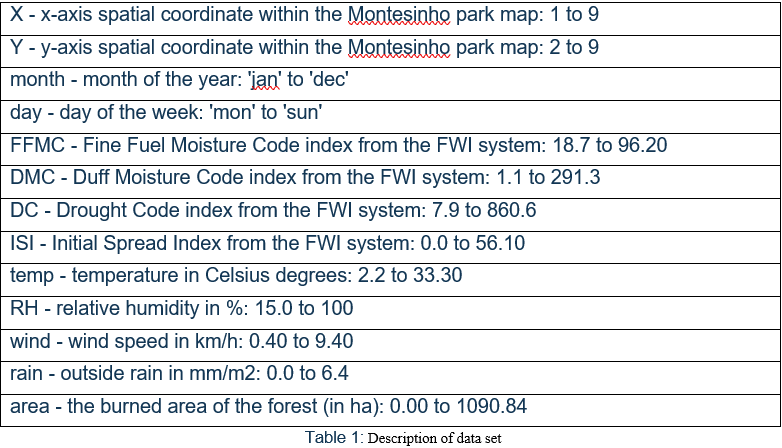
\includegraphics[width=105mm,scale=1.0]{table1.png}}
\end{figure}

\section{OVERVIEW OF METHODS}
\subsection{Multilayer Perceptron(MLP)}
An MLP is a type of artificial neural network model and also feed-forward process. This model maps a set of input data over a set of convenient outputs. An MLP includes multiple layers of nodes in a coordinated graph and each layer is completely connected to the following one. Each node is a neuron with a nonlinear activation function except the input nodes. This method uses a handled learning technique. This technique is named as back propagation in order to train the network. MLP is an alteration of the standard linear perceptron and can recognize inseparable data. An MLP has a form as given Fig. 2.
\begin{figure}[htb!]
\centerline
{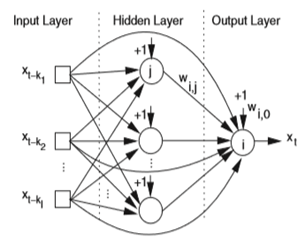
\includegraphics[width=70mm,scale=1.0]{mlp.png}}
\caption{A typical MLP structure}
\end{figure}

\subsection{Levenberg-Marquardt Algorithm(LM)}
LM algorithm is a recursive method. It determines a multivariate function’s minimum value such as summing squares of this functions. It indicates a general method for least squares (LS) questions which are non-linear. LM is formed by combination of Gauss-Newton (GM) and steepest descents (SD) technique. If the obtained solution is not close to correct solution, then LM acts such as SD; that is, slower, but most probably find the correct answer. However, if the obtained solution is very close to the target one, then LM acts as GN.The algorithm of LM is given by Fig. 3. 
\begin{figure}[htb!]
\centerline
{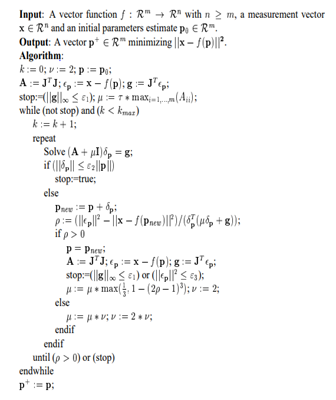
\includegraphics[width=70mm,scale=1.0]{lm.png}}
\caption{LM algorithm}
\end{figure}


\section{Source Code Explanation}
First of all, We read the data-set file which name is 'forestfires.csv'. And then we took attributes namely 'temp','RH','Wind','Rain' and 'Area'. We split the data-set into 2 part 'test' and 'training'. 30\% of the data is for test and the rest of the data is for training. We used 'Multi Layer Perceptron' model with 2 hidden layer size (16,8). Also we used 'relu' function as an activation function.
Then we fitted train part. Then we defined a function to calculate 'rmse (Root Means Square Error)'. We predicted test and training data, called 'RMSE' function with respect to each of them. Then, we defined  'Levenberg-Marquardt' function name as 'model' and do the needed calculation inside of it. And also we defined 'func' to call it in 'least\_squares'. Lastly, we printed Least Squares Model with Levenberg-Marquardt algorithm respect to rmse. RMSE’s for predicting forest fires is shown the table below.

\begin{table}[htb!]
\centering
\begin{tabular}{|c|c|}
\hline
Models                         & RMSE   \\ \hline
MLP(One Hidden Layer + relu)   & 68.280 \\ \hline
MLP(Two Hidden Layer + relu)   & 61.711 \\ \hline
MLP(Three Hidden Layer + relu) & 63.204 \\ \hline
LM                             & 63.576 \\ \hline
\end{tabular}
\end{table}
We took area and month attributes from the data-set to be able to draw in which months had burned area. To do that, we created a dictionary as a 'monthDict'. Then, we put every months on dictionary as keys. We sum up all burned area according to those months. Also, we showed total burned area(in ha). We observed that There is no forest fires on January and November as seen in figure 4.

\begin{figure}[htb!]
\centerline
{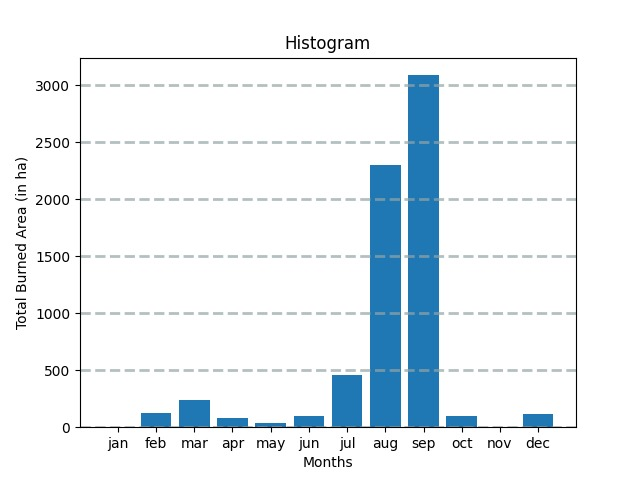
\includegraphics[width=100mm,scale=1.0]{histogram.jpeg}}
\caption{Total Burned Area With Respect to Month }
\end{figure}

At the end, We tried to create a 'heat map' according to 'X' and 'Y' coordinates which is shown in Figure 1.  Firstly, We added all temperatures with respect to  'X' and 'Y' coordinates. Then we counted how many times 'X-Y' repeated (e.g 7-5 (X-Y) is repeated 11 times) and divided total temperature according to its repeated times. We showed it into 'heat map'  as shown in figure 5. Zeros in the heat map means there is no information about that coordinates on the data file(forestfires.csv).

\begin{figure}[htb!]
\centerline
{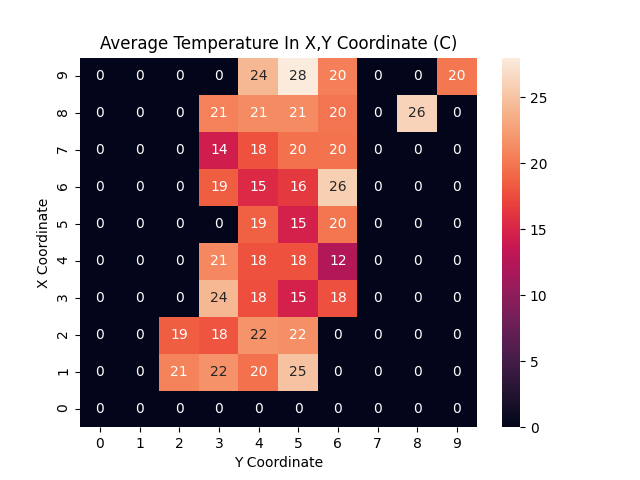
\includegraphics[width=80mm,scale=1.0]{heatMap.png}}
\caption{Heat Map}
\end{figure}


\section{Conclusion}
In conclusion, in this project we learnt to predict the forest fires to decrease the harm that would occur by these fires. One of the most factor for forest fire is alteration on climates; that is, higher temperature or less rain which can be explain with global warming. And also, we learnt how to use 'Multi Layer Perceptron' model which is a type of artificial neural network model and also feed-forward process, and 'Levenberg-Marquardt' algorithm which is a recursive method. We observed that when we were using 'logistic' activation, we got wrong  differences between errors. Because logistic activation was always giving us as a error '0' or '1'. Then, according to our search, we changed activation as a 'relu'. Although errors are independent, error always close to each other between 'Lm','MLP' algorithms. Also, We drew total burned area depends on each month. At the end we drew the average temperature with respect to coordinate of the forest.


\nocite{*}
\bibliographystyle{plain}
\bibliography{references}
\begin{thebibliography}{9}

\texttt{[1]	P. Cortez and A. D. J. R. Morais. "A data mining approach to predict forest fires using meteorological data." In J. Neves, M. F. Santos and J. Machado Eds., New Trends in Artificial Intelligence, Proceedings of the 13th EPIA 2007 - Portuguese Conference on Artificial Intelligence, December, Guimarães, Portugal, pp. 512-523, 2007. APPIA, ISBN-13 978-989-95618-0-9.2007.}
\\
\\
\texttt{[2]	B. C. Arrue, A. Ollero, and J. M. De Dios. "An intelligent system for false alarm reduction in infrared forest-fire detection." IEEE Intelligent Systems and Their Applications, vol. 15 no. 3, pp. 64-73, 2000.}
\\
\\
\texttt{[3]	D. T. Bui, Q. T. Bui, Q. P,.Nguyen, B. Pradhan, H. Nampak, and P. T. Trinh. "A hybrid artificial intelligence approach using GIS-based neural-fuzzy inference system and particle swarm optimization for forest fire susceptibility modeling at a tropical area." Agricultural and forest meteorology, vol.233 pp. 32-44, 2017. }
\\
\\
\texttt{[4]	H. Soliman, K. Sudan, and A. Mishra. "A smart forest-fire early detection sensory system: Another approach of utilizing wireless sensor and neural networks." In Sensors, 2010 IEEE, pp. 1900-1904. IEEE, 2010.}
\\
\\
\texttt{[5]	E. E. Maeda, A. R. Formaggio, Y. E. Shimabukuro, G. F. B. Arcoverde, and M. C. Hansen. "Predicting forest fire in the Brazilian Amazon using MODIS imagery and artificial neural networks." International Journal of Applied Earth Observation and Geoinformation, vol.11 no. 4 pp. 265-272, 2009.}
\end{thebibliography}
\end{document}